
%%%%%%%%%%%%%%%%%%%%%%%%%%%%%%%%%%%%%%%%%%%%%%%%%%%%%%%%%%%%%%%%%%%%%
%% This is a (brief) model paper using the achemso class
%% The document class accepts keyval options, which should include
%% the target journal and optionally the manuscript type.
%%%%%%%%%%%%%%%%%%%%%%%%%%%%%%%%%%%%%%%%%%%%%%%%%%%%%%%%%%%%%%%%%%%%%
\documentclass[journal=jcisd8,manuscript=article]{achemso}

%%%%%%%%%%%%%%%%%%%%%%%%%%%%%%%%%%%%%%%%%%%%%%%%%%%%%%%%%%%%%%%%%%%%%
%% Place any additional packages needed here.  Only include packages
%% which are essential, to avoid problems later.
%%%%%%%%%%%%%%%%%%%%%%%%%%%%%%%%%%%%%%%%%%%%%%%%%%%%%%%%%%%%%%%%%%%%%
\usepackage{chemformula} % Formula subscripts using \ch{}
\usepackage[T1]{fontenc} % Use modern font encodings
\usepackage{hyperref} % For hyperlinks in the PDF
\usepackage{url}
\usepackage[version=4]{mhchem} % Formula subscripts using \ce{}
\usepackage{booktabs} % For formal tables
\usepackage{siunitx}  % 可选但推荐，用于处理单位和数字对齐
\usepackage{amsmath}
\usepackage{graphicx}
%%%%%%%%%%%%%%%%%%%%%%%%%%%%%%%%%%%%%%%%%%%%%%%%%%%%%%%%%%%%%%%%%%%%%
%% If issues arise when submitting your manuscript, you may want to
%% un-comment the next line.  This provides information on the
%% version of every file you have used.
%%%%%%%%%%%%%%%%%%%%%%%%%%%%%%%%%%%%%%%%%%%%%%%%%%%%%%%%%%%%%%%%%%%%%
%%\listfiles

%%%%%%%%%%%%%%%%%%%%%%%%%%%%%%%%%%%%%%%%%%%%%%%%%%%%%%%%%%%%%%%%%%%%%
%% Place any additional macros here.  Please use \newcommand* where
%% possible, and avoid layout-changing macros (which are not used
%% when typesetting).
%%%%%%%%%%%%%%%%%%%%%%%%%%%%%%%%%%%%%%%%%%%%%%%%%%%%%%%%%%%%%%%%%%%%%
\newcommand*\mycommand[1]{\texttt{\emph{#1}}}

%%%%%%%%%%%%%%%%%%%%%%%%%%%%%%%%%%%%%%%%%%%%%%%%%%%%%%%%%%%%%%%%%%%%%
%% Meta-data block
%% ---------------
%% Each author should be given as a separate \author command.
%%
%% Corresponding authors should have an e-mail given after the author
%% name as an \email command. Phone and fax numbers can be given
%% using \phone and \fax, respectively; this information is optional.
%%
%% The affiliation of authors is given after the authors; each
%% \affiliation command applies to all preceding authors not already
%% assigned an affiliation.
%%
%% The affiliation takes an option argument for the short name.  This
%% will typically be something like "University of Somewhere".
%%
%% The \altaffiliation macro should be used for new address, etc.
%% On the other hand, \alsoaffiliation is used on a per author basis
%% when authors are associated with multiple institutions.
%%%%%%%%%%%%%%%%%%%%%%%%%%%%%%%%%%%%%%%%%%%%%%%%%%%%%%%%%%%%%%%%%%%%%

\author{Wenyuan Zhao}
% \affiliation{Graduate School of Chemical Sciences and Engineering, Hokkaido University, Sapporo, Japan}
\affiliation{Department of Chemistry, Faculty of Science, Hokkaido University, Sapporo 060-0810, Japan}

\author{Xianzhu Zhong}
\author{Simeng Wang}
\author{ashikeri}
\author{mohanmode}
\author{Jouffery Xiaer}
\author{Yirui Peng}
\author{Aiichiro Nagaki}
\email{nagaki@sci.hokudai.ac.jp}
% Kita 10-jo, Nishi 8-chome, Kita-ku, Sapporo 060-0810 (Japan)
% \affiliation{Department of Chemistry, Faculty of Science, Hokkaido University, Sapporo 060-0810, Japan}
\affiliation{Department of Chemistry, Faculty of Science, Hokkaido University, Sapporo 060-0810, Japan}

%%%%%%%%%%%%%%%%%%%%%%%%%%%%%%%%%%%%%%%%%%%%%%%%%%%%%%%%%%%%%%%%%%%%%
%% The document title should be given as usual. Some journals require
%% a running title from the author: this should be supplied as an
%% optional argument to \title.
%%%%%%%%%%%%%%%%%%%%%%%%%%%%%%%%%%%%%%%%%%%%%%%%%%%%%%%%%%%%%%%%%%%%%
\title[FlowFigTabMiner]
  {FlowFigTabMiner: Multimodal Extraction of Structured Flow Chemistry Data from Figures, Tables, and Text Enables Organolithium Lifetime Prediction}

%%%%%%%%%%%%%%%%%%%%%%%%%%%%%%%%%%%%%%%%%%%%%%%%%%%%%%%%%%%%%%%%%%%%%
%% Some journals require a list of abbreviations or keywords to be
%% supplied. These should be set up here, and will be printed after
%% the title and author information, if needed.
%%%%%%%%%%%%%%%%%%%%%%%%%%%%%%%%%%%%%%%%%%%%%%%%%%%%%%%%%%%%%%%%%%%%%
% \abbreviations{IR,NMR,UV}
\keywords{Flow Chemistry, Multimodal Data Extraction, YOLO, Organolithium, Intermediate Lifetime, Literature Mining}

%%%%%%%%%%%%%%%%%%%%%%%%%%%%%%%%%%%%%%%%%%%%%%%%%%%%%%%%%%%%%%%%%%%%%
%% The manuscript does not need to include \maketitle, which is
%% executed automatically.
%%%%%%%%%%%%%%%%%%%%%%%%%%%%%%%%%%%%%%%%%%%%%%%%%%%%%%%%%%%%%%%%%%%%%
\begin{document}

%%%%%%%%%%%%%%%%%%%%%%%%%%%%%%%%%%%%%%%%%%%%%%%%%%%%%%%%%%%%%%%%%%%%%
%% The "tocentry" environment can be used to create an entry for the
%% graphical table of contents. It is given here as some journals
%% require that it is printed as part of the abstract page. It will
%% be automatically moved as appropriate.
%%%%%%%%%%%%%%%%%%%%%%%%%%%%%%%%%%%%%%%%%%%%%%%%%%%%%%%%%%%%%%%%%%%%%
\begin{tocentry}
% The surrounding frame is 9\,cm by 3.5\,cm。

%% A TOC figure needs to be added.
\begin{minipage}{9cm}

\includegraphics[width=8cm]{figures/TOC.PNG} 
\end{minipage}

\end{tocentry}

%%%%%%%%%%%%%%%%%%%%%%%%%%%%%%%%%%%%%%%%%%%%%%%%%%%%%%%%%%%%%%%%%%%%%
%% The abstract environment will automatically gobble the contents
%% if an abstract is not used by the target journal.
%%%%%%%%%%%%%%%%%%%%%%%%%%%%%%%%%%%%%%%%%%%%%%%%%%%%%%%%%%%%%%%%%%%%%
\begin{abstract}
Quantitative reaction data in flow chemistry literature is predominantly stored in figures (yield-vs-residence-time heatmaps) and tables (with embedded molecular structure images), formats inaccessible to conventional text mining.
We present FlowFigTabMiner, a fully automated multimodal pipeline that chains Florence-2 for figure/table detection, four custom YOLO models for element segmentation, PaddleOCR for text recognition, MolNexTR for image-to-SMILES conversion, and LLM adjudication for evidence integration.
On a 10-figure/10-table benchmark, the pipeline achieves an overall extraction F1 of 0.838, outperforming Gemini~3.1~Pro (0.833) and Claude~Sonnet~4.6 (0.806), with a dominant advantage on figure extraction (F1~=~0.892 vs 0.575/0.561).
Applied to 125 organolithium flow chemistry publications, the pipeline constructs a 1{,}470-row kinetics dataset---the first with flow-condition coverage (residence time, temperature, yield).
Kinetic modeling of the extracted yield-vs-$t_R$ data yields decomposition activation energies ($E_a$) for 14 organolithium intermediates spanning nearly four orders of magnitude in half-life.
A Hammett correlation ($E_a = -48.5\sigma + 36.1$~kJ/mol, $r = -0.979$) and a Taft steric correlation (log~$t_{1/2} = -1.13 E_s + 0.04$, $r = -0.969$) enable quantitative prediction of ArLi intermediate stability from substituent constants alone.
Arrhenius extrapolation to batch conditions ($-78$~\si{\celsius}, 600~s) predicts intermediate survival within 3\% of experimental yields, validating the extracted kinetic parameters for reactor selection.
\end{abstract}

%%%%%%%%%%%%%%%%%%%%%%%%%%%%%%%%%%%%%%%%%%%%%%%%%%%%%%%%%%%%%%%%%%%%%
%% Start the main part of the manuscript here.
%%%%%%%%%%%%%%%%%%%%%%%%%%%%%%%%%%%%%%%%%%%%%%%%%%%%%%%%%%%%%%%%%%%%%
\section{INTRODUCTION}

% --- P1: AI for chemistry + data bottleneck (KEPT, lightly revised) ---
Recent advances in generative artificial intelligence, particularly large language models (LLMs), are expanding the applications of machine learning in chemical engineering\cite{schweidtmann2024generative,D5CS00146C,D4SC03921A,boiko2023autonomous,doi:10.1021/acs.oprd.3c00229}.
These models have demonstrated significant potential across diverse tasks, such as assisting with process flow diagrams\cite{aicheasdas}, predicting thermochemical and kinetic properties\cite{tomme2025machine}, aiding process development\cite{ruan2024automatic}, and optimizing reaction conditions or yields\cite{doi:10.1021/acs.jcim.2c01085,doi:10.1021/acs.jcim.0c01234,schwaller2021prediction,D2SC06041H}.
However, a primary bottleneck limits the broader application of these AI models: the lack of high-quality, large-scale training datasets.\cite{tomme2025machine,gartner2024data,chen2024autotemplate}
In response to this challenge, significant efforts are underway to improve data standardization and accessibility.
For example, \citeauthor{doi:10.1021/jacs.1c09820} have pioneered the development of reaction databases and defined standardized formats to promote effective data sharing and reuse\cite{doi:10.1021/acs.jcim.3c00607}.
\citeauthor{jacs_mof} successfully addressed the data scarcity challenge by employing a chain of advanced LLMs to mine over 40,000 articles, constructing a comprehensive, structured dataset for metal-organic frameworks (MOFs)\cite{jacs_mof}.

% --- P2: Specific gap for flow chemistry — data in FIGURES and TABLES (REVISED) ---
A critical gap persists for flow chemistry data in particular.
Advancements in laboratory automation, including high-throughput experimentation (HTE)\cite{lu2024roboticized,li2023deep} and flow chemistry\cite{D5DD00129C,ashikari2025real,adamo2016demand}, can produce standardized experimental data at scale.
However, the published flow chemistry literature, while rich in information, stores critical reaction parameters not only in text but also in \textit{figures} (yield-vs-residence-time curves, temperature--time heatmaps) and \textit{tables} (often containing molecular structure images rather than text-based SMILES).
Existing structured databases such as USPTO and the Open Reaction Database (ORD)\cite{doi:10.1021/jacs.1c09820} lack flow-specific parameters---residence time, flow rate, and reactor geometry---that are essential for process optimization.\cite{Deadman_2025}
As a result, publicly available, structured databases for flow chemistry remain remarkably scarce, directly hindering the development of robust machine learning models tailored for continuous manufacturing.

% --- P3: Prior work on chemical information extraction (KEPT) ---
Over the past few decades, various methods have been developed to extract structured information from unstructured chemical literature.
Leveraging natural language processing (NLP) techniques to build systems that can automatically and effectively process lengthy chemical texts,
including scientific literature or patents, in order to extract key information has received widespread attention\cite{KURGAN_MUSILEK_2006}.
Supervised learning models like Google’s  BERT  language  model\cite{BERT} and its domain-specific variants such as SciBERT\cite{SciBERT}, ChemBERTa\cite{ChemBERTa},
BioBERT\cite{BioBERT}, and MatSciBERT\cite{MatSciBERT} have been successfully applied to various chemical text mining tasks.

For instance, OPSIN \cite{lowe_2012} serves as an early exemplar, utilizing a heuristic-based method that underscores the potential benefits of applying NLP to chemical data extraction.
ChemDataExtractor \cite{ChemDataExtractor} pioneered an automated approach to extract chemical information from scientific literature by integrating NLP and machine learning techniques.
Subsequently, ChemRxnBERT \cite{Guo2022-tk} harnessed the power of pre-training on chemical literature to foster a deeper understanding of chemical context.
More recently, OpenChemIE \cite{doi:10.1021/acs.jcim.4c00572} introduced an open-source toolkit that automatically extracts chemical reaction data by integrating information from text, tables, and figures.
Xiang et al. \cite{Xiang2025-dp} presented a workflow that employs a local LLMs combined with multi-step prompt engineering to automatically extract synthesis parameters for on-surface reactions.
However, it does not capture process-level information such as reactor types or influencing process parameters.
Pan et al. \cite{Pan2025-sj} introduced Chat-microreactor, an LLM-based assistant that extracts fluidic properties and microchannel dimensions from literature to train machine learning models for classifying multiphase flow patterns (e.g., dripping, jetting).
Nevertheless, this tool is explicitly prompted to ignore chemical reaction data and therefore does not extract critical process development parameters such as catalyst, temperature, or yield.
Critically, all of these tools operate exclusively on text, leaving the quantitative data encoded in scientific figures and molecular structures embedded in tables entirely untapped.

% --- P4: VLM limitations for quantitative figure reading (NEW) ---
Vision-Language Models (VLMs) such as GPT-4V, Gemini, and Claude have emerged as promising multimodal extractors capable of ``seeing’’ figures and tables directly.\cite{openai2024gpt4technicalreport,google2025gemini25flashlite}
However, our evaluation reveals that these models hallucinate coordinates when reading dense scatter plots, with F1 scores dropping below 0.36 on complex heatmaps and multi-series figures (Section~\ref{sec:benchmark}).
VLMs approximate rather than precisely read pixel positions, leading to systematic errors in quantitative data extraction.
Furthermore, commercial safety guardrails frequently block legitimate flow chemistry queries involving high-energy reactions (e.g., nitration, azides) or hazardous conditions, severely limiting their utility for process development literature.\cite{röttger2024xstesttestsuiteidentifying}
No existing end-to-end system addresses the full pipeline from PDF ingestion through figure/table detection, element segmentation, coordinate extraction, and molecular structure recognition to a structured database.

% --- P5: Our contribution (NEW) ---
Herein, we introduce \textbf{FlowFigTabMiner}, a fully automated multimodal pipeline for extracting structured process data from flow chemistry literature.
The framework chains Florence-2 for figure/table detection, four custom-trained YOLO models for element segmentation, the Table Transformer (TATR) for cell structure recognition, PaddleOCR for text extraction, MolNexTR for image-to-SMILES molecular structure conversion, and LLM-based adjudication for evidence merging.
Three key advances are demonstrated:
(1) YOLO-based coordinate mapping from scientific figures that surpasses state-of-the-art VLMs, achieving an extraction F1 of 0.892 compared to 0.575 for Gemini 3.1 Pro and 0.561 for Claude Sonnet 4.6;
(2) integrated table extraction with molecular structure recognition, enabling SMILES conversion from structure images;
(3) construction of a 1{,}470-row organolithium kinetics dataset and a 1{,}267-row scope table dataset from 125 publications---the first with flow-condition coverage (residence time, temperature, yield).
We further demonstrate the dataset’s chemical utility by extracting decomposition activation energies ($E_a$) for 14 organolithium intermediates and establishing quantitative Hammett ($E_a$ vs $\sigma$, $r = -0.979$) and Taft ($t_{1/2}$ vs $E_s$, $r = -0.969$) correlations that predict ArLi intermediate stability from substituent constants.
The kinetic parameters are validated by Arrhenius extrapolation to independent batch scope data, confirming quantitative predictive accuracy.
The pipeline, models, dataset, and a cloud-deployed web tool are open-sourced.

\section{RESULTS AND DISCUSSION}

%%%%%%%%%%%%%%%%%%%%%%%%%%%%%%%%%%%%%%%%%%%%%%%%%%%%%%%%%%%%%%%%%%%%%
%% 2.1 Pipeline Architecture
%%%%%%%%%%%%%%%%%%%%%%%%%%%%%%%%%%%%%%%%%%%%%%%%%%%%%%%%%%%%%%%%%%%%%
\subsection{Pipeline Architecture}

% --- P1: Overview of the 4-layer design (~150 words) --- TO BE FILLED
% - Input Layer: PDF ingestion + TF-ID (Florence-2-base) detects figures and
%   tables on each page, saving cropped images
% - Processing Layer: three parallel tracks (figure, table, text)
% - Algorithm Layer: LLM adjudication merging all evidence
% - Output Layer: normalized JSON / CSV database

% --- P2: Figure processing track (~200 words) --- TO BE FILLED
% - Step 1: YOLO macro segmentation (v11m-fig-seg, 6 classes)
% - Step 2: YOLO micro detection (v11m-fig-sca, 4 classes)
% - Step 3: Coordinate mapping — OCR tick labels, build pixel-to-physical
%   axis transforms, map each data_point to (X, Y_Left, Y_Right)
% - Step 4: Legend matching — assign series labels by color/position proximity
% - Handles: scatter plots, line charts, bar charts, heatmaps

% --- P3: Table processing track (~200 words) --- TO BE FILLED
% - Step B1: YOLO table segmentation (v11m-tab-seg, 4 classes)
% - Step B2: YOLO molecule detection (v11s-tab-mol)
% - Step B3: Molecule masking — white fill to prevent OCR interference
% - Step B4: TATR structure recognition — rows, columns, headers -> cell grid
% - Step B5: PaddleOCR for text cells; MolNexTR for molecule cells (image->SMILES)
% - Step B6: CSV assembly with keyword-based relevance filtering

% --- P4: LLM adjudication and cloud deployment (~150 words) --- TO BE FILLED
% - LLM merges figure evidence (JSON), table evidence (CSV), text context
% - Unit normalization, SMILES validation, cross-source deduplication
% - Cloud deployment: 4 microservices on GCP Cloud Run
% - GCS-mounted model weights; public web interface

\begin{figure*}[!ht]
    \centering
    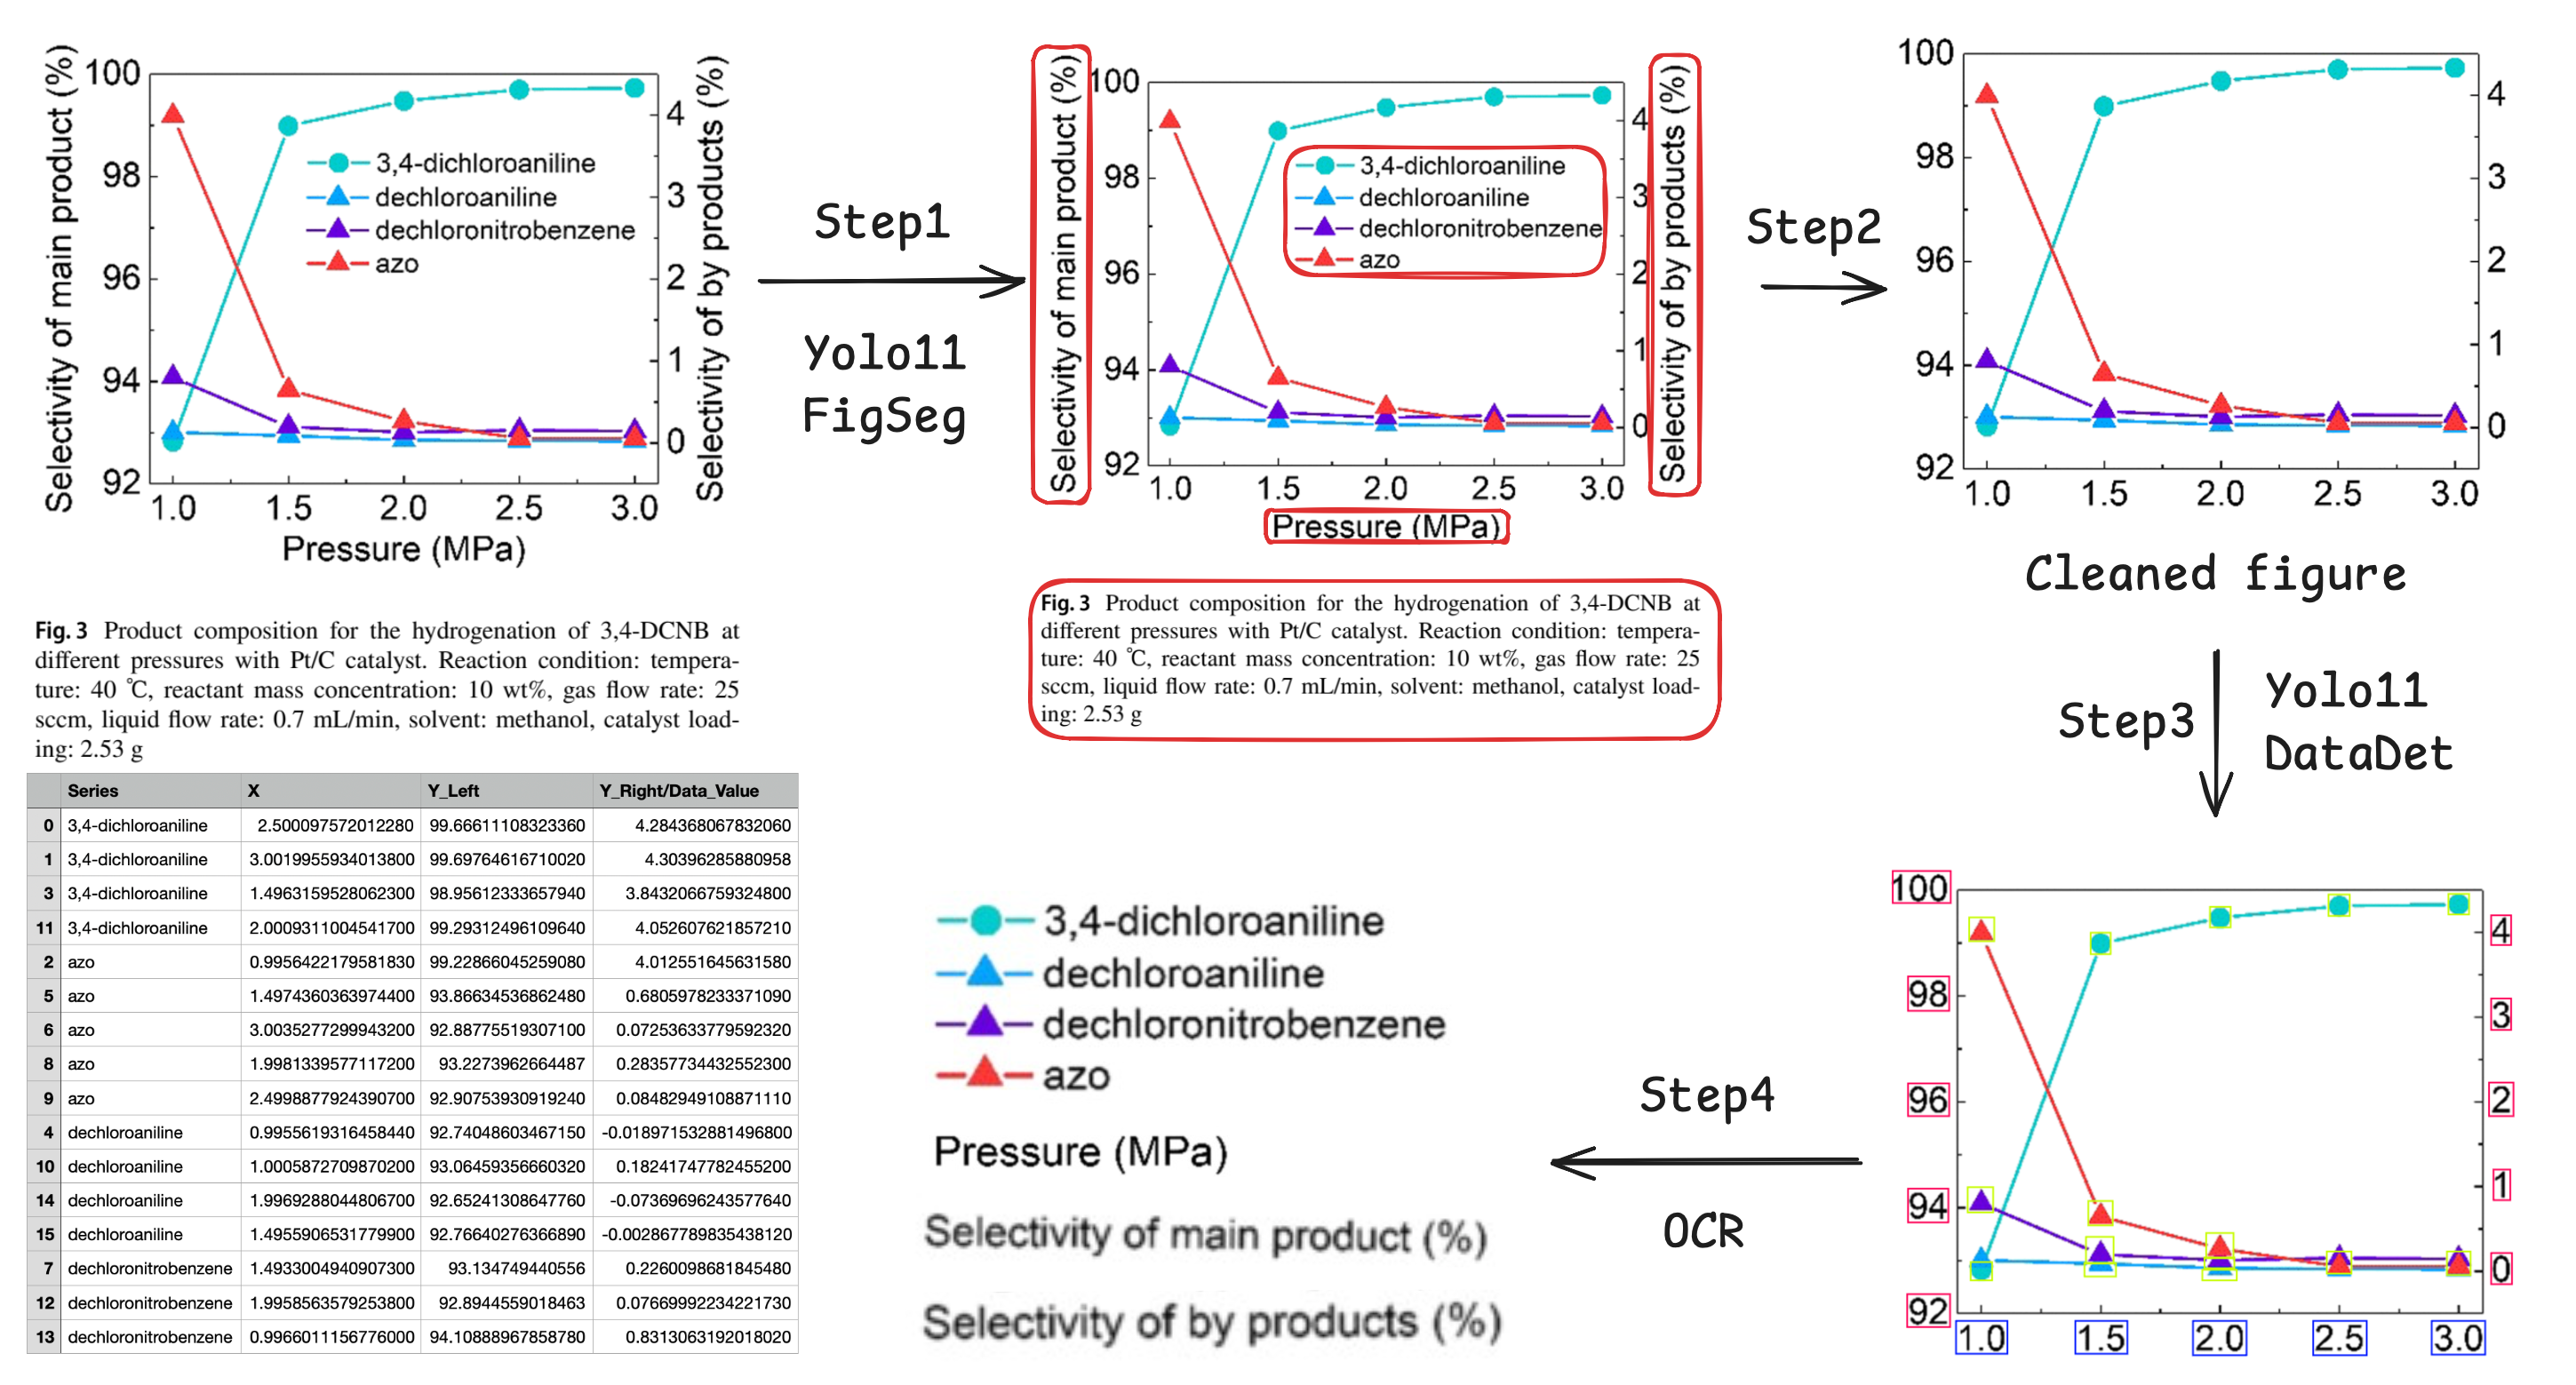
\includegraphics[width=\linewidth]{figures/pipeline-figure.png}
    \caption{Overall architecture of the FlowFigTabMiner pipeline for figure data extraction. The workflow processes PDF documents through TF-ID detection, YOLO-based macro segmentation and micro detection, coordinate mapping, and legend matching to produce structured data points.}
    \label{fig:pipeline-figure}
\end{figure*}

\begin{figure*}[!ht]
    \centering
    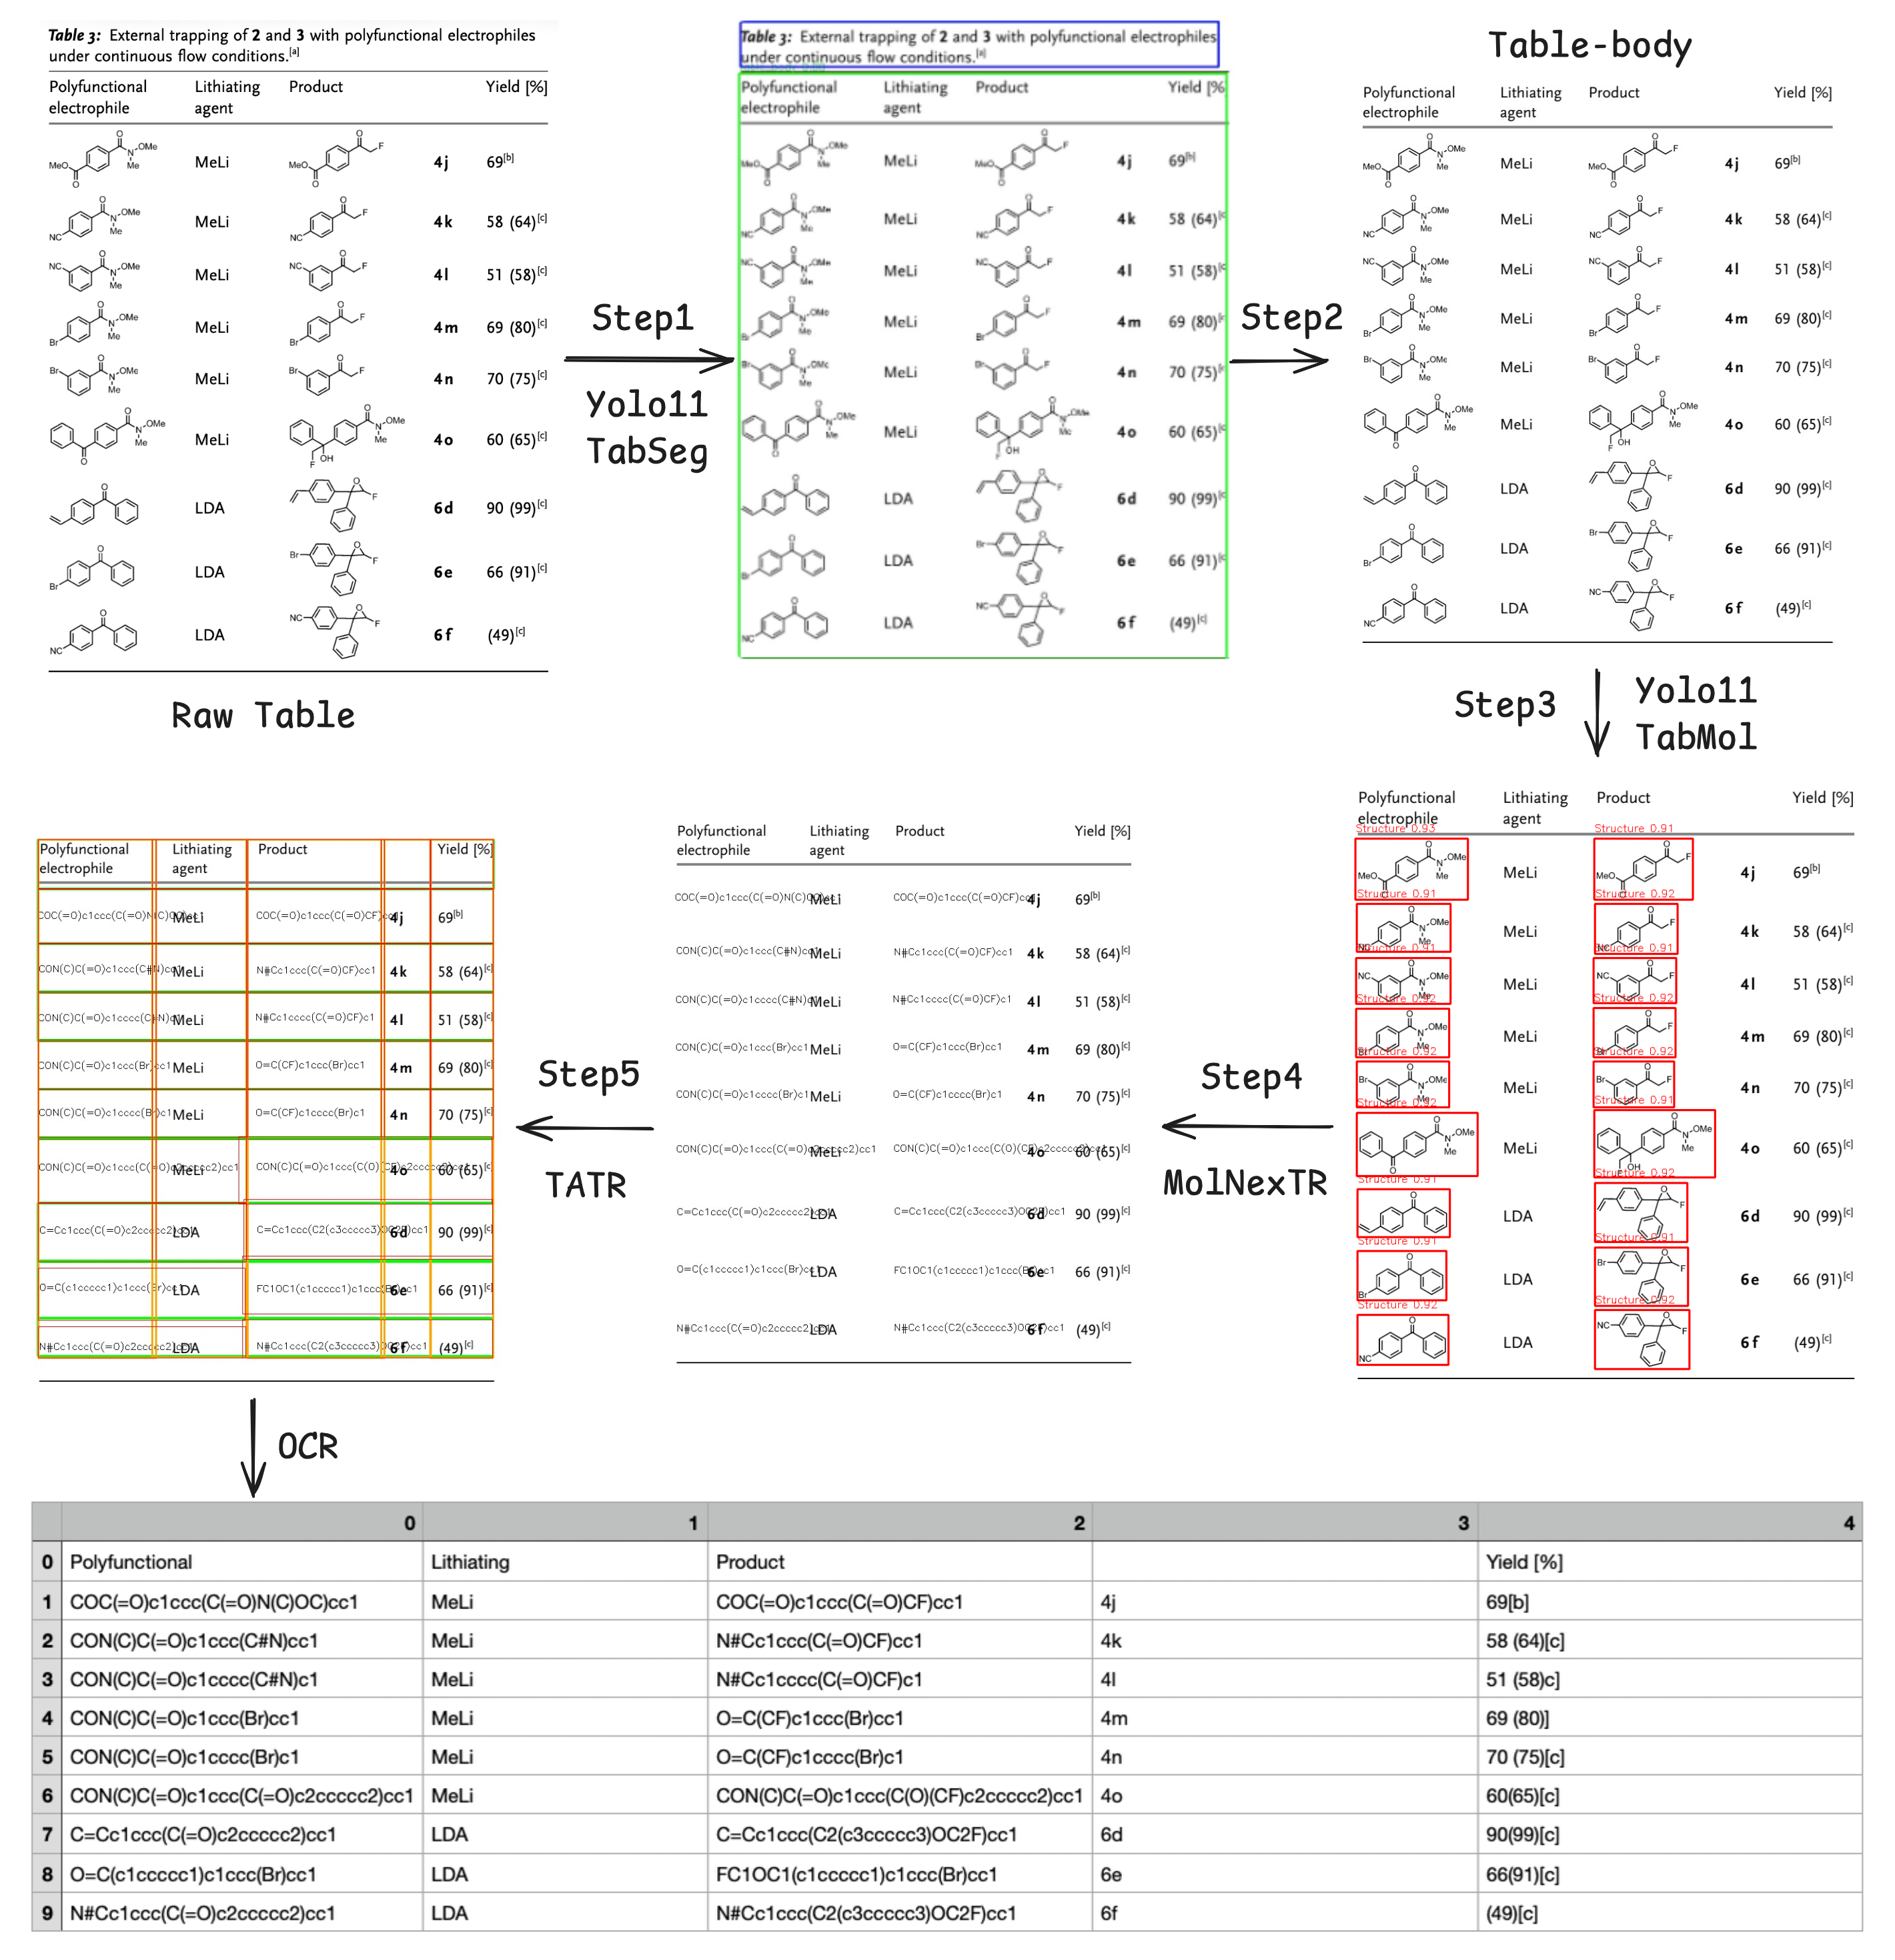
\includegraphics[width=\linewidth]{figures/pipeline-table.png}
    \caption{Table extraction sub-pipeline. YOLO detects table regions and molecular structures; structures are masked before TATR cell detection; PaddleOCR reads text cells while MolNexTR converts structure images to SMILES.}
    \label{fig:pipeline-table}
\end{figure*}

%%%%%%%%%%%%%%%%%%%%%%%%%%%%%%%%%%%%%%%%%%%%%%%%%%%%%%%%%%%%%%%%%%%%%
%% 2.2 YOLO Model Training
%%%%%%%%%%%%%%%%%%%%%%%%%%%%%%%%%%%%%%%%%%%%%%%%%%%%%%%%%%%%%%%%%%%%%
\subsection{YOLO Model Training and Object Detection}

% --- P1: Training data and annotation (~150 words) --- TO BE FILLED
% - Manually annotated chemical figures and tables from flow chemistry papers
% - Four models trained on YOLOv11 architecture (Ultralytics)
% - Model sizes: v11m (medium) for segmentation, v11s (small) for mol detection

% --- P2: Model descriptions and class definitions (~150 words) --- TO BE FILLED
% - v11m-fig-seg: 6 classes (caption, legend, subfigure_marker, target_image,
%   x_axis_title, y_axis_title)
% - v11m-fig-sca: 4 classes (data_point, data_value, x_tick_label, y_tick_label)
% - v11m-tab-seg: 4 classes (table_body, table_caption, table_note, table_scheme)
% - v11s-tab-mol: 1 class (Structure)

% --- P3: Results and discussion (~200 words) --- TO BE FILLED
% - All models achieve mAP50 > 91.7% (Table~\ref{tab:yolo_results})
% - tab-mol highest precision (96.2%): distinctive visual features
% - fig-sca 92.5% mAP50: critical for coordinate mapping
% - fig-seg lowest mAP50-95 (66.9%): axis titles vary in position/font

\begin{table}[htbp]
\centering
\caption{Comparative experimental results of different YOLO models for FlowFigTabMiner. The best performance is indicated in bold.}
\label{tab:yolo_results}
\begin{tabular}{@{}lccccc@{}}
\toprule
\textbf{Models} & \textbf{Precision/\%} & \textbf{Recall/\%} & \textbf{F1 Score/\%} & \textbf{mAP50/\%} & \textbf{mAP50--95/\%} \\ \midrule
v11m-fig-seg  & 88.2 & 91.7 & 89.9 & 91.7 & 66.9 \\
v11m-fig-sca  & 92.1 & 91.9 & 92.0 & 92.5 & 69.3 \\
v11m-tab-seg  & 91.2 & 89.9 & 90.5 & 94.8 & 77.7 \\
v11s-tab-mol  & \textbf{96.2} & \textbf{95.4} & \textbf{95.8} & \textbf{95.6} & \textbf{81.2} \\
\bottomrule
\end{tabular}
\end{table}

\begin{figure}[!ht]
    \centering
    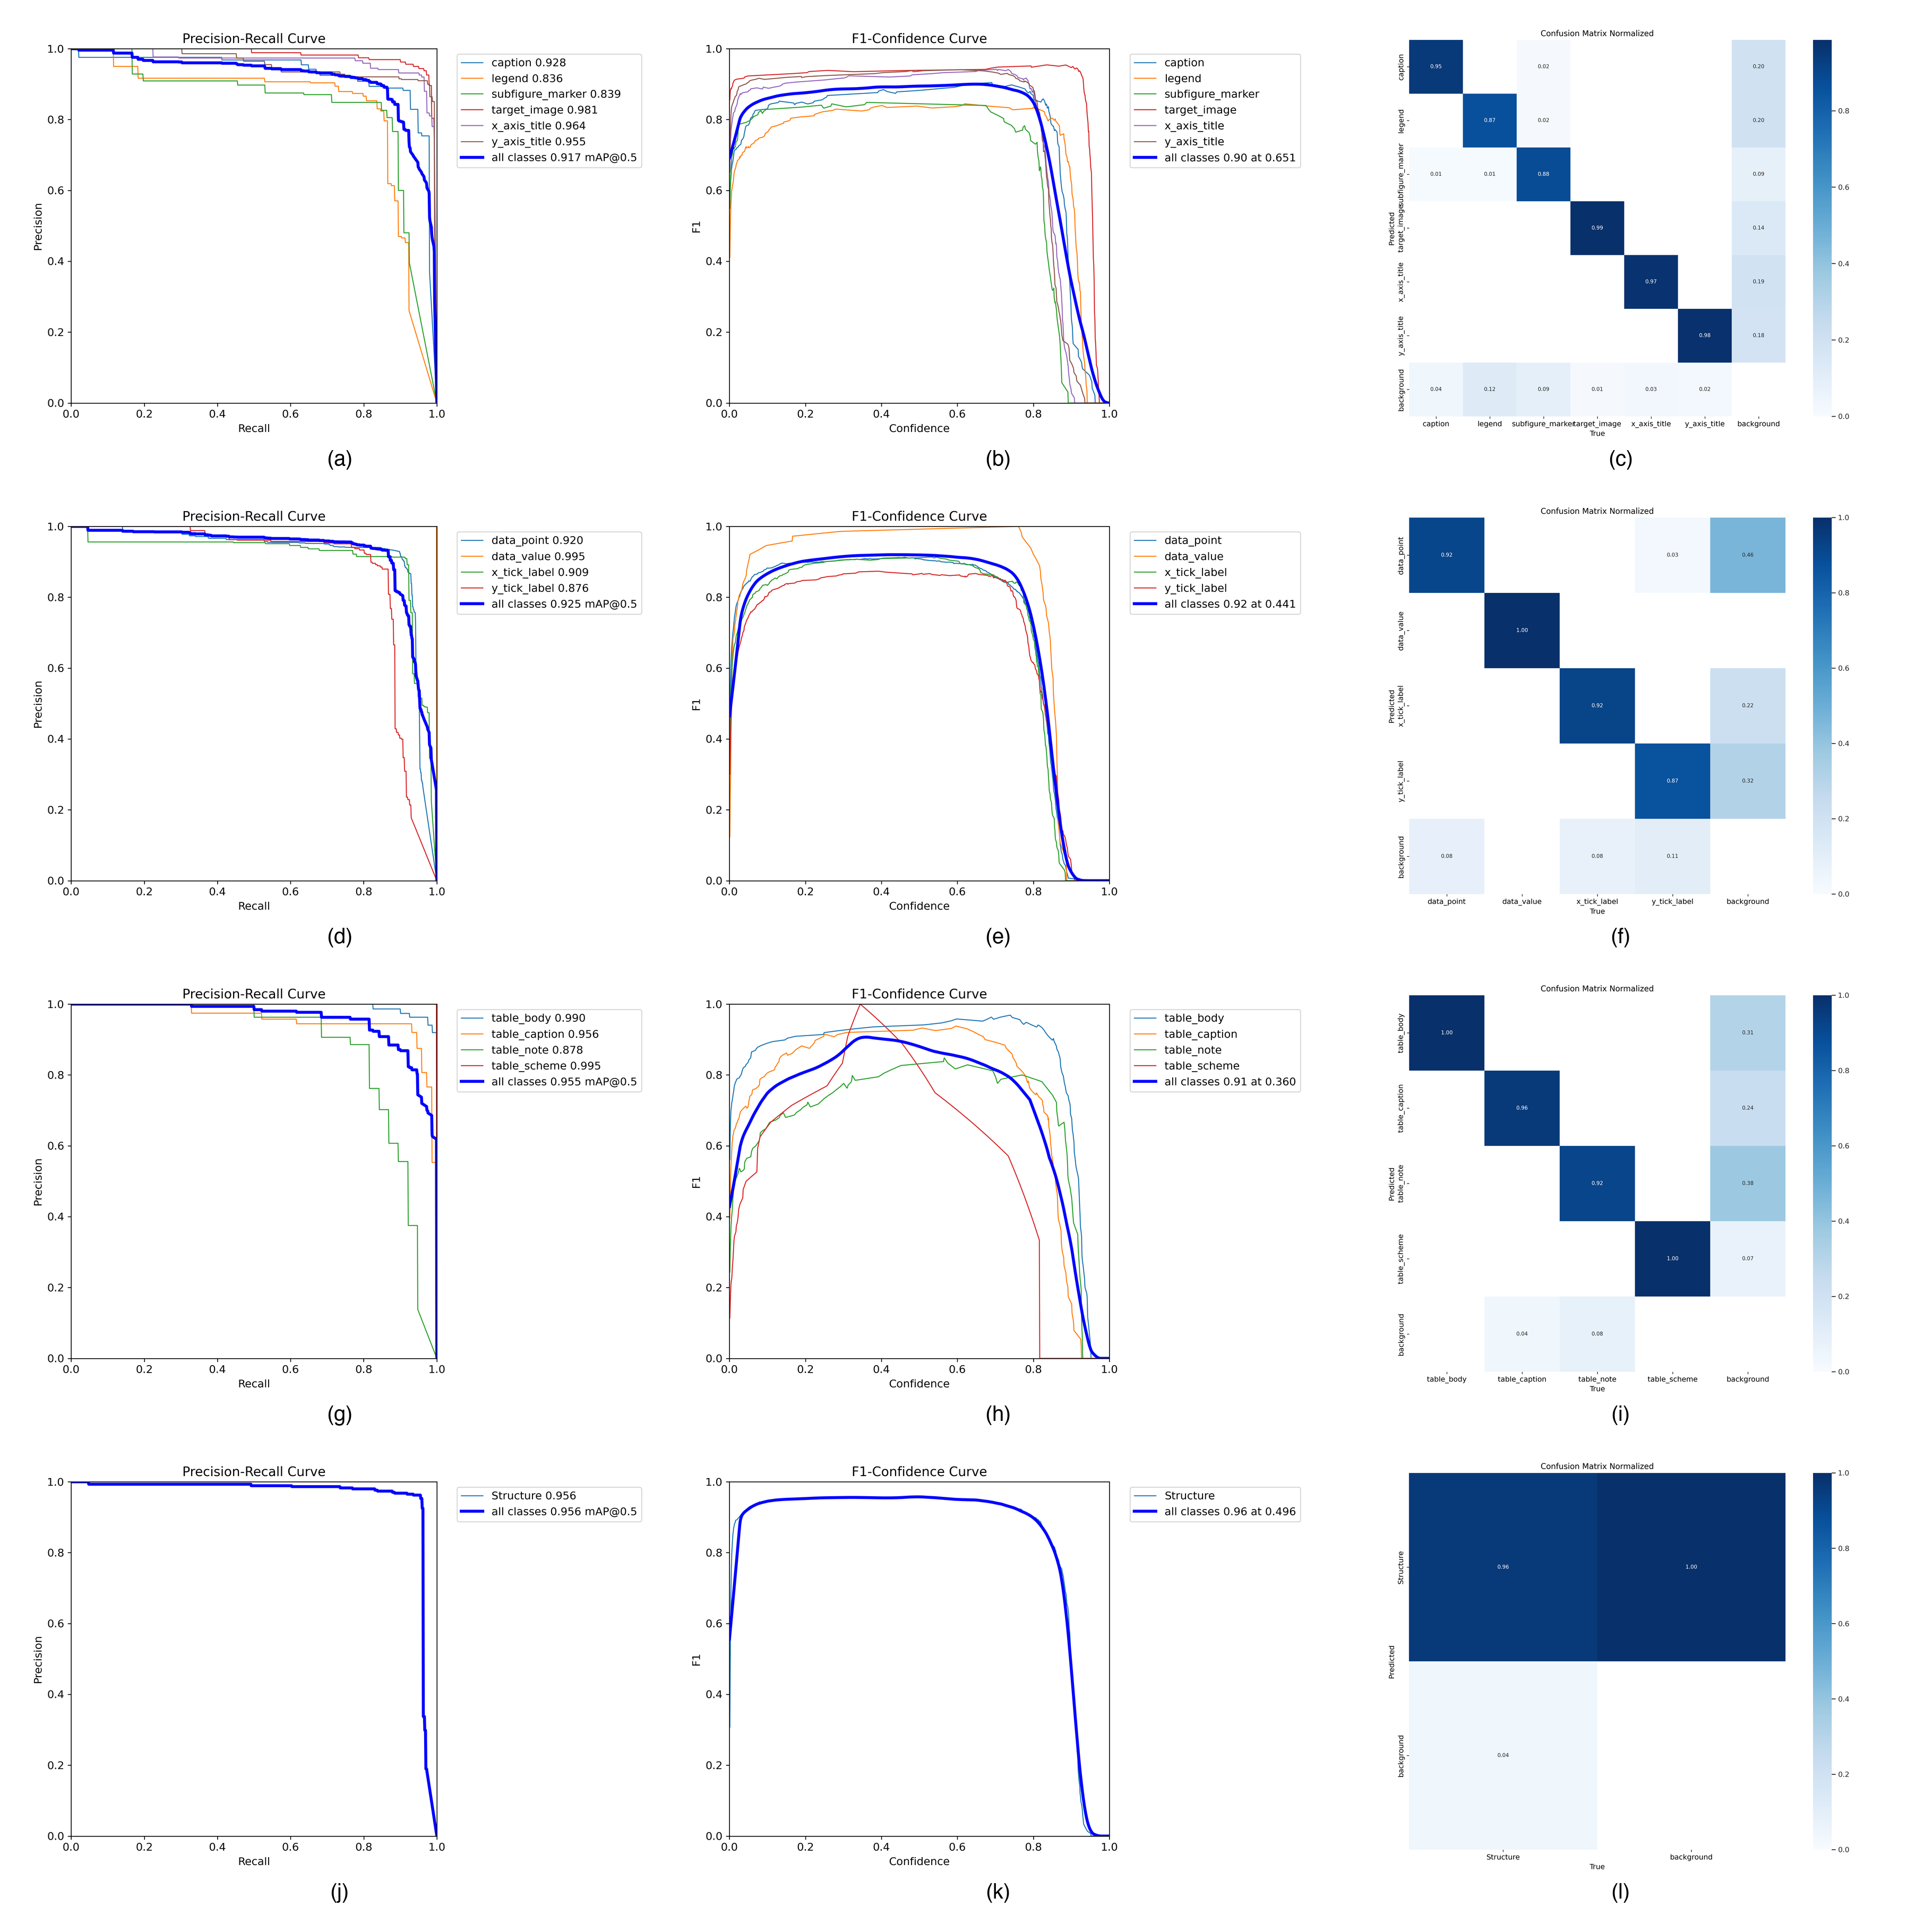
\includegraphics[width=\linewidth]{figures/fig-yolo-results.png}
    \caption{YOLO detection examples. (a)~Figure macro segmentation showing detected axes, legend, and caption regions. (b)~Scatter point detection with bounding boxes on data points and tick labels. (c)~Table segmentation identifying body, caption, and scheme regions. (d)~Molecular structure detection within table cells.}
    \label{fig:yolo-examples}
\end{figure}

%%%%%%%%%%%%%%%%%%%%%%%%%%%%%%%%%%%%%%%%%%%%%%%%%%%%%%%%%%%%%%%%%%%%%
%% 2.3 Three-Way Benchmark vs VLMs
%%%%%%%%%%%%%%%%%%%%%%%%%%%%%%%%%%%%%%%%%%%%%%%%%%%%%%%%%%%%%%%%%%%%%
\subsection{Three-Way Benchmark: Pipeline vs.\ State-of-the-Art VLMs}
\label{sec:benchmark}

% --- P1: Evaluation methodology (~150 words) --- TO BE FILLED
% - 10 figures (F1-F10) + 10 tables (T1-T10); VLMs on F1-F5 + T1-T5
% - Three systems: FlowFigTabMiner, Gemini 3.1 Pro, Claude Sonnet 4.6
% - GT: manual annotation by doctoral researchers
% - Matching: greedy nearest-neighbor with 5% tolerance (figures);
%   exact match (tables); RDKit validity (SMILES)

% --- P2: Figure extraction results (~150 words) --- TO BE FILLED
% - Pipeline F1=0.892 (P=0.876, R=0.932) on F1-F5
% - Gemini F1=0.575, Claude F1=0.561
% - Pipeline 55% higher F1 than best VLM
% - VLMs collapse on F3 (heatmap, 0.36) and F5 (dense scatter, 0.19)
% - Root cause: VLMs approximate coordinates; YOLO reads precise pixels

% --- P3: Table extraction results (~150 words) --- TO BE FILLED
% - Pipeline F1=0.827, Gemini F1=0.98, Claude F1=0.99
% - VLMs clearly superior for table OCR
% - Pipeline limitations: TATR row/column misalignment (T3, T4)

% --- P4: SMILES extraction results (~100 words) --- TO BE FILLED
% - Pipeline: F1=0.795 (MolNexTR image->SMILES)
% - Gemini: F1=0.944, Claude: F1=0.867
% - Different tasks: pipeline converts structure IMAGES (harder);
%   VLMs read SMILES TEXT already in tables

% --- P5: Overall results and key insight (~150 words) --- TO BE FILLED
% - Overall: Pipeline F1=0.838 > Gemini 0.833 > Claude 0.806
% - Pipeline wins BECAUSE of dominant figure extraction
% - Key insight: strengths are complementary
% - Cost: pipeline fully automated; VLMs require per-image API costs

\begin{table}[htbp]
\centering
\caption{Three-way comparison: FlowFigTabMiner vs.\ VLMs on 5 figures and 5 tables.}
\label{tab:three-way-comparison}
\begin{tabular}{llccc}
\toprule
\textbf{Task} & \textbf{Metric} & \textbf{FlowFigTabMiner} & \textbf{Gemini 3.1 Pro} & \textbf{Claude Sonnet 4.6} \\
\midrule
Figure (F1--F5) & Precision & \textbf{0.876} & 0.531 & 0.513 \\
                & Recall    & \textbf{0.932} & 0.659 & 0.651 \\
                & F1        & \textbf{0.892} & 0.575 & 0.561 \\
\midrule
Table (T1--T5)  & Precision & 0.843 & 0.98  & \textbf{0.99} \\
                & Recall    & 0.814 & 0.98  & \textbf{0.99} \\
                & F1        & 0.827 & 0.98  & \textbf{0.99} \\
\midrule
SMILES (T1--T5) & Precision & 0.925 & \textbf{0.944} & 0.893 \\
                & Recall    & 0.697 & \textbf{0.944} & 0.843 \\
                & F1        & 0.795 & \textbf{0.944} & 0.867 \\
\midrule
\textbf{Overall} & Precision & \textbf{0.881} & 0.818 & 0.799 \\
                & Recall    & 0.814 & \textbf{0.861} & 0.828 \\
                & F1        & \textbf{0.838} & 0.833 & 0.806 \\
\bottomrule
\end{tabular}
\end{table}

% TODO: Create Figure — per-figure and per-table F1 bar chart
% Data source: eval/three_way_comparison.json
%\begin{figure}[!ht]
%    \centering
%    \includegraphics[width=\linewidth]{figures/fig-three-way-bar.png}
%    \caption{Per-sample F1 score comparison. (a)~Figure extraction (F1--F5): the pipeline consistently outperforms both VLMs. (b)~Table extraction (T1--T5): VLMs achieve near-perfect accuracy.}
%    \label{fig:three-way-bar}
%\end{figure}

%%%%%%%%%%%%%%%%%%%%%%%%%%%%%%%%%%%%%%%%%%%%%%%%%%%%%%%%%%%%%%%%%%%%%
%% 2.4 Organolithium Dataset Construction
%%%%%%%%%%%%%%%%%%%%%%%%%%%%%%%%%%%%%%%%%%%%%%%%%%%%%%%%%%%%%%%%%%%%%
\subsection{Organolithium Dataset Construction}

% --- P1: Domain choice and corpus assembly (~150 words) --- TO BE FILLED
% - Organolithium flow chemistry: unstable intermediates demand precise tR control
% - 125 papers via keyword search, spanning 2005-2024

% --- P2: Dataset statistics (~150 words) --- TO BE FILLED
% - 3,195 rows; Structure 15.1%, Outcome 61.3%, Yield 49.3%,
%   Temp 71.5%, Time 56.7%, Solvent 70.9%, Flow 85.1%
% - 2,884 modeling-ready rows; 1,688 with non-null residence time

% --- P3: Comparison with existing datasets (~200 words) --- TO BE FILLED
% - USPTO-LLM: 6,073 rows, 100% structure, 0% outcome, 0% flow vars
% - ORD: 43,004 rows, 99.9% structure, 44.3% yield, 0% flow vars
% - Our dataset = ONLY one with flow-condition coverage
% - Unique: heatmap-derived data (249 rows from 12 figure groups)

% --- P4: Data quality (~100 words) --- TO BE FILLED
% - Human-in-the-loop verification by doctoral researchers
% - Conservative SMILES enrichment (exact name-to-SMILES from ORD)
% - 15+ organolithium reaction types classified

\begin{table*}[t]
\centering
\small
\caption{Comparison of the three organolithium datasets. Our dataset is the only one with flow-condition coverage and substantial outcome data, making it uniquely suited for flow process optimization.}
\label{tab:dataset-comparison}
\begin{tabular}{p{2.8cm}p{2.8cm}p{1.1cm}p{0.8cm}p{0.9cm}p{1.0cm}p{0.9cm}p{0.9cm}p{0.9cm}p{0.9cm}p{0.9cm}p{0.9cm}p{0.9cm}p{0.9cm}}
\hline
Dataset & Source type & Rows & Sources & Struct. & Outcome & Yield & Temp. & Time & Solvent & Catalyst & Flow & Batch & Model-ready \\
\hline
Our dataset & literature-derived curated dataset & 3195 & 125 & 15.1\% & 61.3\% & 49.3\% & 71.5\% & 56.7\% & 70.9\% & 27.1\% & 85.1\% & 4.5\% & 34.7\% \\
USPTO-LLM organolithium & patent-derived transformed corpus & 6073 & 2 & 100.0\% & 0.0\% & 0.0\% & 97.6\% & 97.4\% & 93.9\% & 1.8\% & 0.0\% & 0.0\% & 0.0\% \\
ORD organolithium & public structured reaction database & 43004 & 4 & 99.9\% & 100.0\% & 44.3\% & 44.7\% & 65.2\% & 74.7\% & 4.8\% & 0.0\% & 0.0\% & 23.9\% \\
\hline
\end{tabular}
\end{table*}

% TODO: Create/select Figure — dataset overview
%\begin{figure}[!ht]
%    \centering
%    \includegraphics[width=\linewidth]{figures/fig-dataset-overview.png}
%    \caption{Organolithium dataset overview. (a)~Field completeness comparison across our dataset, USPTO-LLM, and ORD. (b)~Reaction type composition of the 3,195-row dataset.}
%    \label{fig:dataset-overview}
%\end{figure}

%%%%%%%%%%%%%%%%%%%%%%%%%%%%%%%%%%%%%%%%%%%%%%%%%%%%%%%%%%%%%%%%%%%%%
%% 2.5 ML Lifetime Prediction
%%%%%%%%%%%%%%%%%%%%%%%%%%%%%%%%%%%%%%%%%%%%%%%%%%%%%%%%%%%%%%%%%%%%%
\subsection{Organolithium Intermediate Lifetime Prediction}

Organolithium intermediates are kinetically unstable species whose lifetime governs the optimal residence time ($t_R$) and, consequently, the choice between batch, flow, or flash chemistry reactors.\cite{Yoshida2008flash}
Yield-vs-$t_R$ heatmaps, ubiquitous in flow chemistry publications, encode this kinetic information in their shape: a rising phase (formation-limited), a peak, and a decay phase (decomposition-limited).
Extracting quantitative kinetics from these figures is precisely the task for which FlowFigTabMiner was designed (figure F1~=~0.892).

\subsubsection{Half-life extraction from yield decay curves}

From 20 papers containing yield-vs-$t_R$ heatmaps, the pipeline extracted 1{,}470 data points covering 14 organolithium intermediates, each measured at 2--6 temperature levels with 5--8 residence times per level.
Residence times were manually corrected from heatmap axis annotations (logarithmic scales), and yields were independently verified against a YOLO-based OCR pipeline (99.6\% agreement, 734/737 exact matches).

For each (intermediate, temperature) pair, the data were fitted to a competing first-order kinetics model:
\begin{equation}\label{eq:yield-approx}
\text{yield}(t_R) = y_{\max} \left(1 - e^{-k_f t_R}\right) e^{-k_d t_R}
\end{equation}
where $k_f$ and $k_d$ are the formation and decomposition rate constants, respectively, and $t_{1/2} = \ln 2 / k_d$.
A total of 76 (intermediate, $T$) groups were fitted, of which 53 exhibited measurable decay.

\subsubsection{Arrhenius analysis}

For each intermediate, the temperature dependence of $k_d$ was modeled by the Arrhenius equation:
\begin{equation}\label{eq:arrhenius}
\ln(k_d) = \ln(A) - \frac{E_a}{RT}
\end{equation}
Activation energies ranged from 4.8~kJ/mol (\textit{m}-lithiobenzonitrile) to 65.4~kJ/mol (\textit{o}-bromoaryllithium), and half-lives at $-40$~\si{\celsius} spanned nearly four orders of magnitude: from 3.3~ms (\textit{o}-iodoaryllithium) to 51.9~s (\textit{tert}-butyl \textit{o}-(lithio)benzoate).
Arrhenius fits yielded $R^2 > 0.95$ for 10 of 14 intermediates.

Three mechanistically distinct classes emerged from the $E_a$ landscape:
(i)~conjugation-stabilized ArLi ($E_a$ = 4.8--41.3~kJ/mol, 8 species), where the electron-withdrawing group delocalizes the carbanion;
(ii)~$\alpha$-elimination carbenoids ($E_a$ = 16.2--49.2~kJ/mol, 3 species);
(iii)~benzyne-elimination ArLi ($E_a$ = 59.7--65.4~kJ/mol, 2 species), proceeding through concerted 1,2-elimination.

\subsubsection{Hammett correlation for meta/para-substituted ArLi}

For the subset of conjugation-stabilized ArLi bearing \textit{meta} or \textit{para} substituents, the decomposition activation energy correlated strongly with the Hammett substituent constant:
\begin{equation}\label{eq:hammett}
E_a = -48.5\sigma + 36.1 \quad (r = -0.979,\ p = 0.021,\ n = 4)
\end{equation}
The negative slope indicates that stronger electron-withdrawing groups (higher $\sigma$) lower the activation barrier.
Paradoxically, these intermediates are \textit{more} stable because the pre-exponential factor $\ln A$ decreases even faster---a manifestation of enthalpy--entropy compensation ($\ln A = 0.63 E_a - 4.6$, $r = 0.987$).
The isokinetic temperature ($T_{\mathrm{iso}} = 191$~K $\approx -82$~\si{\celsius}) is close to the standard organolithium working temperature ($-78$~\si{\celsius}, dry ice/acetone), explaining why cryogenic conditions effectively equalize the stability of structurally diverse intermediates.

\subsubsection{Taft steric correlation for ortho-substituted ArLi}

The four \textit{ortho}-alkoxycarbonyl ArLi intermediates (R = Me, Et, \textit{i}Pr, \textit{t}Bu) share identical Hammett $\sigma$ values (0.45) but differ dramatically in stability.
Their half-lives correlate with the Taft steric parameter $E_s$:
\begin{equation}\label{eq:taft}
\log(t_{1/2}) = -1.13\,E_s + 0.04 \quad (r = -0.969,\ p = 0.031,\ n = 4)
\end{equation}
The \textit{tert}-butyl ester ($E_s = -1.54$) is 86$\times$ more stable than the methyl ester ($E_s = 0.00$) at $-40$~\si{\celsius} ($t_{1/2}$ = 51.9~s vs 602~ms).
Notably, the same \ce{CO2^{t}Bu} group at the \textit{ortho} position is 10.8$\times$ more stable than at \textit{para} ($t_{1/2}$ = 51.9~s vs 4.8~s), demonstrating that steric shielding of the C--Li bond outweighs electronic stabilization for \textit{ortho} substituents.

These results establish a two-parameter framework for ArLi intermediate stability: Hammett $\sigma$ for \textit{meta}/\textit{para} positions and Taft $E_s$ for \textit{ortho} positions.

\subsubsection{Validation by Arrhenius extrapolation to batch conditions}

To test whether the extracted kinetic parameters are quantitatively predictive beyond the original flow conditions, we extrapolated the Arrhenius parameters of the four \textit{ortho}-ester ArLi intermediates from the flow heatmap regime ($-70$ to $20$~\si{\celsius}, 0.003--25~s) to batch conditions ($-78$~\si{\celsius}, 600~s).
The predicted survival fractions were compared with independently measured batch yields from scope tables in the same publication (Table~\ref{tab:batch-validation}).

\begin{table}[htbp]
\centering
\caption{Arrhenius extrapolation validation: predicted intermediate survival at $-78$~\si{\celsius}, 600~s versus measured batch yields.}
\label{tab:batch-validation}
\begin{tabular}{@{}lcccc@{}}
\toprule
\textbf{Ester R} & \textbf{$E_a$ (kJ/mol)} & \textbf{$t_{1/2}$ ($-78$~\si{\celsius})} & \textbf{Predicted survival} & \textbf{Batch yield} \\
\midrule
\textit{t}Bu & 26.8 & 766~s & 58\% & 61\% \\
\textit{i}Pr & 38.0 & 257~s & 20\% & 12\% \\
Et            & 41.3 & 116~s & 3\%  & 0\% \\
Me            & 36.5 & 24~s  & 0\%  & 0\% \\
\bottomrule
\end{tabular}
\end{table}

The \textit{tert}-butyl ester prediction (58\%) matches the experimental yield (61\%) within 3 percentage points.
For the ethyl and methyl esters, both prediction and experiment agree that the intermediates decompose completely under batch conditions.
This close agreement---across a 100~\si{\celsius} temperature extrapolation and a 24$\times$ residence time extrapolation---validates the heatmap-derived Arrhenius parameters as quantitatively useful for reactor selection.

\subsubsection{Predictive application}

To close the prediction loop, three \textit{para}-substituted aryllithiums not present in the training set were selected for experimental validation (Table~\ref{tab:predictions}).
The predicted $E_a$ values are obtained from Equation~\ref{eq:hammett}; $\ln A$ from the compensation relation; and $t_{1/2}$ from Equation~\ref{eq:arrhenius}.

\begin{table}[htbp]
\centering
\caption{Hammett-predicted kinetic parameters for three untested ArLi intermediates.}
\label{tab:predictions}
\begin{tabular}{@{}lccccl@{}}
\toprule
\textbf{Intermediate} & \textbf{$\sigma$} & \textbf{$E_a^{\mathrm{pred}}$ (kJ/mol)} & \textbf{$t_{1/2}$ ($-40$~\si{\celsius})} & \textbf{$t_{1/2}$ ($0$~\si{\celsius})} & \textbf{Regime} \\
\midrule
\textit{p}-\ce{CF3}-PhLi & $+0.54$ & 9.9  & 23~s   & 11~s    & batch-compatible \\
\textit{p}-F-PhLi        & $+0.06$ & 33.2 & 1.7~s  & 140~ms  & flow \\
\textit{p}-\ce{CH3}-PhLi & $-0.17$ & 44.3 & 500~ms & 17~ms   & flash \\
\bottomrule
\end{tabular}
\end{table}

The three substrates span the entire reactor regime classification: \textit{p}-\ce{CF3}-PhLi (strong EWG, low $E_a$) is predicted to be stable enough for batch operation; \textit{p}-F-PhLi requires continuous flow; and \textit{p}-\ce{CH3}-PhLi (weak EDG, high $E_a$) demands flash chemistry conditions at temperatures above $-20$~\si{\celsius}.
These predictions are currently being validated experimentally using a T-mixer microreactor setup with MeOH quench (8 residence times $\times$ 4--5 temperatures per substrate).

%\begin{figure*}[!ht]
%    \centering
%    \includegraphics[width=\linewidth]{figures/ml-results.png}
%    \caption{Kinetic analysis and structure--activity relationships for organolithium intermediates. (a)~Hammett plot: $E_a$ vs $\sigma$ for meta/para ArLi (filled circles) and benzyne outliers (open triangles), with three predicted validation targets. (b)~Arrhenius plots for 14 intermediates. (c)~Enthalpy--entropy compensation ($\ln A$ vs $E_a$). (d)~Stability ranking at $-40$~\si{\celsius} with reactor regime zones.}
%    \label{fig:ml-results}
%\end{figure*}

%%%%%%%%%%%%%%%%%%%%%%%%%%%%%%%%%%%%%%%%%%%%%%%%%%%%%%%%%%%%%%%%%%%%%
%% 3. CONCLUSIONS
%%%%%%%%%%%%%%%%%%%%%%%%%%%%%%%%%%%%%%%%%%%%%%%%%%%%%%%%%%%%%%%%%%%%%
\section{CONCLUSIONS}

We have presented FlowFigTabMiner, the first fully automated multimodal pipeline for extracting structured process data from flow chemistry literature.
On a 10-figure/10-table benchmark, the pipeline achieves an overall extraction F1 of 0.838, outperforming Gemini~3.1~Pro (0.833) and Claude~Sonnet~4.6 (0.806), with a decisive advantage on quantitative figure extraction (F1~=~0.892 vs 0.575/0.561).

Applied to 125 organolithium flow chemistry publications, the pipeline constructed a 1{,}470-row kinetics dataset and a 1{,}267-row scope table dataset---the first with flow-condition coverage.
From yield-vs-$t_R$ heatmaps alone, we extracted decomposition activation energies for 14 organolithium intermediates spanning nearly four orders of magnitude in half-life (3.3~ms to 51.9~s at $-40$~\si{\celsius}).

Two quantitative structure--stability relationships emerged from the extracted data:
(1)~A Hammett correlation ($E_a = -48.5\sigma + 36.1$~kJ/mol, $r = -0.979$) for \textit{meta}/\textit{para}-substituted ArLi;
(2)~A Taft steric correlation ($\log t_{1/2} = -1.13 E_s + 0.04$, $r = -0.969$) for \textit{ortho}-ester ArLi.
Neither correlation has been previously reported for organolithium decomposition kinetics, despite the underlying qualitative trends being well established.
The kinetic parameters were validated by Arrhenius extrapolation to batch conditions ($-78$~\si{\celsius}, 600~s), where the predicted \textit{tert}-butyl ester survival (58\%) matched the experimental yield (61\%) within 3 percentage points.

The combined Hammett--Taft framework provides a practical tool for reactor selection: given only the Hammett $\sigma$ or Taft $E_s$ of the substituent, one can predict $E_a$, $t_{1/2}$ at any temperature, and the appropriate reactor regime (batch, flow, or flash).
Three validation substrates (\textit{p}-\ce{CF3}-, \textit{p}-F-, and \textit{p}-\ce{CH3}-bromobenzene) have been selected for experimental confirmation.

Limitations include the small number of intermediates (14) and the moderate sample size for both Hammett ($n = 4$) and Taft ($n = 4$) correlations.
The pipeline architecture is domain-agnostic and can be extended to other organometallic systems (Grignard, organozinc) or domains where quantitative data is locked in scientific figures.
% - All code, models, dataset, and web tool open-sourced

\section{EXPERIMENTAL SECTION}

\subsection{Pipeline Implementation and Deployment}
% (~250 words) --- TO BE FILLED
% - Python 3.10, PyTorch 2.8.0
% - TF-ID: Florence-2-base (HuggingFace yifeihu/TF-ID-base)
% - YOLO: Ultralytics YOLOv11 (v11m/v11s); 1024px input
% - TATR: Microsoft Table Transformer v1.1
% - PaddleOCR: PaddlePaddle 3.x, PP-OCRv5_server
% - MolNexTR: image-to-SMILES (1.06 GiB model)
% - LLM adjudication: cloud LLM via API
% - Cloud: 4 microservices on GCP Cloud Run
%   Memory: tfid 16Gi (GPU), figure 8Gi, table 16Gi
% [PLACEHOLDER — to be filled with FlowFigTabMiner implementation details]

\subsection{YOLO Model Training}
% (~200 words) --- TO BE FILLED
% - Training data: manually annotated chemical figures/tables
% - YOLOv11m (fig-seg, fig-sca, tab-seg), YOLOv11s (tab-mol)
% - Hyperparams: [epochs, batch size, lr, image size, augmentation]

\subsection{Coordinate Mapping Algorithm}
% (~150 words) --- TO BE FILLED
% - Input: YOLO-detected positions + OCR tick labels
% - Linear pixel-to-physical transform per axis
% - Special cases: dual Y-axes, log scales, heatmaps
% - Legend matching via color proximity

\subsection{Evaluation Protocol}
\label{sec:eval}
% (~200 words) --- TO BE FILLED
% - 10 figures + 10 tables; VLMs on F1-F5 + T1-T5
% - GT: manual annotation by doctoral researchers
% - Figure matching: greedy NN, 5% tolerance
% - SMILES: RDKit validity
% - Overall: macro-average of Figure F1, Table F1, SMILES F1
Standard metrics were calculated based on True Positives (TP), False Positives (FP), and False Negatives (FN):
\begin{equation}
\text{Precision} = \frac{\mathrm{TP}}{\mathrm{TP}+\mathrm{FP}}
\end{equation}
\begin{equation}
\text{Recall} = \frac{\mathrm{TP}}{\mathrm{TP}+\mathrm{FN}}
\end{equation}
\begin{equation}
\text{F1} = 2 \times \frac{\text{Precision} \times \text{Recall}}{\text{Precision} + \text{Recall}}
\end{equation}
\begin{equation}
mAP_{50} = \frac{1}{N} \sum_{i=1}^N AP_{50, i}
\end{equation}
\begin{equation}
mAP_{50\text{--}95} = \frac{1}{N} \sum_{i=1}^N \frac{1}{K} \sum_{j=1}^K AP_{i, j}
\end{equation}

\subsection{Dataset Construction and Normalization}
% (~150 words) --- TO BE FILLED
% - 125 papers via keyword filtering
% - Normalization: temp->C, time->s, flow->mL/min
% - Conservative SMILES enrichment from ORD
% - Doctoral researcher spot-checking

\subsection{Kinetic Modeling}
Yield-vs-$t_R$ data extracted from 20 papers (1{,}470 data points, 14 intermediates) were fitted using \texttt{scipy.optimize.curve\_fit} to the competing kinetics model (Equation~\ref{eq:yield-approx}) for each (intermediate, temperature) pair, yielding the decomposition rate constant $k_d$ and half-life $t_{1/2} = \ln 2 / k_d$.
A total of 76 fits were obtained (53 with measurable decay, 23 formation-only).
For each intermediate, $\ln(k_d)$ values at 2--6 temperatures were fitted to the Arrhenius equation (Equation~\ref{eq:arrhenius}) via linear regression, giving the activation energy $E_a$ and pre-exponential factor $\ln A$.
Hammett $\sigma$ constants were taken from Hansch, Leo, and Taft (1991); Taft $E_s$ values from Taft (1956).
Hammett and Taft correlations were fitted by ordinary least squares with $p$-values from two-sided $t$-tests.
Arrhenius extrapolation to batch conditions used $k_d(T) = \exp[\ln A - E_a/(RT)]$ and survival fraction $= \exp(-k_d \cdot t)$.

\section{ASSOCIATED CONTENT}
\subsection{Data Availability Statement}
\label{dataset}
\begin{itemize}
  \item The source code for the \textbf{FlowFigTabMiner} pipeline is publicly available at \href{https://github.com/wzjeh/FlowFigTabMiner}{\url{https://github.com/wzjeh/FlowFigTabMiner}}.
  \item The trained YOLO models and MolNexTR weights are available on \href{https://huggingface.co/wyzhaoc}{Hugging Face}.
  \item The organolithium kinetics dataset (1{,}470 rows) and scope table dataset (1{,}267 rows) are provided as CSV in the repository.
  \item A cloud-deployed web tool is accessible at [URL].
\end{itemize}

\begin{suppinfo}
The Supporting Information is available free of charge at
\url{https://pubs.acs.org/}.
\begin{itemize}
  \item Full per-figure and per-table benchmark breakdown (F1--F10, T1--T10) (PDF)
  \item SMILES extraction detailed results and inter-system comparison (PDF)
  \item Standardized VLM prompts for figure and table extraction (PDF)
  \item Step-by-step extraction walkthrough examples (PDF)
  \item Complete list of 125 papers in the organolithium corpus (PDF)
  \item Phase A--C kinetic modeling full results (PDF)
  \item Cloud deployment architecture and specifications (PDF)
  \item YOLO training curves and class distribution details (PDF)
\end{itemize}
\end{suppinfo}


\section{AUTHOR INFORMATION}
\subsection{Corresponding Author}
Aiichiro Nagaki -- Department of Chemistry, Faculty of Science, Hokkaido University, Sapporo 060-0810, Japan; orcid.org/0000-0002-8264-6205; Email: nagaki@sci.hokudai.ac.jp

\subsection{Authors}
% Wenyuan Zhao -- Department of Chemistry, Faculty of Science, Hokkaido University, Sapporo 060-0810, Japan; orcid.org/0009-0009-7235-3562


% \subsection{Author Contributions}


\subsection{Notes}
The authors declare no competing financial interest.


%%%%%%%%%%%%%%%%%%%%%%%%%%%%%%%%%%%%%%%%%%%%%%%%%%%%%%%%%%%%%%%%%%%%%
%% The "Acknowledgement" section can be given in all manuscript
%% classes.  This should be given within the "acknowledgement"
%% environment, which will make the correct section or running title.
%%%%%%%%%%%%%%%%%%%%%%%%%%%%%%%%%%%%%%%%%%%%%%%%%%%%%%%%%%%%%%%%%%%%%
\begin{acknowledgement}% 已完成
The authors thank the Support for Pioneering Research Initiated by the Next Generation (SPRING) at Hokkaido University (JPMJSP2119) and JSPS KAKENHI (JP20KK0121; JP21H01936) for their financial support. 
This work was also supported by AMED BINDS (PJ22230021), NEDO (PJ22240036), the Japan Keirin Autorace Foundation, and the Takahashi Industrial and Economic Foundation.
\end{acknowledgement}



%%%%%%%%%%%%%%%%%%%%%%%%%%%%%%%%%%%%%%%%%%%%%%%%%%%%%%%%%%%%%%%%%%%%%
%% The appropriate \bibliography command should be placed here.
%% Notice that the class file automatically sets \bibliographystyle
%% and also names the section correctly.
%%%%%%%%%%%%%%%%%%%%%%%%%%%%%%%%%%%%%%%%%%%%%%%%%%%%%%%%%%%%%%%%%%%%%
\bibliography{achemso-demo}

\end{document}
